\chapter{Data and analysis}
\label{cap:metodos}

The preceding chapter established the observables through which collinear spin
correlations can be accessed. Following that, this chapter describes how they are
measured in practice and presents the data on which this analysis is built, the
software environment in which it runs, and the sequence of steps that leads from the
raw available events to the azimuthal distributions of Chapter \ref{cap:resultados}.
The goal of this chapter is to reveal all the steps necessary to make this analysis,
securing reproducibility. That said, enough detail is given, and the code used is
available publicly in \cite{Mendonca:CMSJetSubstructure}, 
so that the analysis can be repeated in full from public inputs alone.

The chapter is organised as follows. Section~\ref{sec:opendata} introduces the
CERN Open Data initiative and the principles that make an analysis of this kind
possible outside the experimental collaborations. Section~\ref{sec:cms} describes
the relevant features of the CMS detector, and Section~\ref{sec:dataset} the data
format and the specific dataset used. Section~\ref{sec:pipeline} presents the
analysis pipeline, from the extraction of jet constituents to the computation of
the spin observables. Section~\ref{sec:flavour} describes the flavour selection
that isolates the $g \to q\bar{q}$ channel, and Section~\ref{sec:systematics}
assesses the systematic uncertainties affecting the measurement.

\section{CERN Open Data}
\label{sec:opendata}

The data analysed in this work were obtained through the CERN Open Data
Portal~\cite{CERNOpenData}, the platform through which the LHC experiments
release reconstructed collision data and the associated simulation to the public.
Launched in 2014, the portal was the first initiative of its kind in high-energy
physics, and it has since grown into a major repository holding data from
the ALICE, ATLAS, CMS and LHCb collaborations. The first releases came from the
CMS experiment, and it is CMS data that this work uses.

The CERN Open Data Portal does not provide detector output but data at the same level
of reconstruction used in collaborations' own published analysis. These datasets
include physics objects such as jets, tracks and reconstructed particles, with the
calibration already applied and run quality information required to use them correctly.
Alongside the collision data, the portal also releases the corresponding Monte Carlo simulations,
the software environment necessary to analyse the datasets and documentation describing their
format and content. All this features of the portal make it possible for any user to
use their data for their own analysis and interpret the results.

The importance of this portal in this work is twofold. First, as made clear in this
chapter's introduction, it makes the measurement reproducible. Every input from 
the collision and respective simulated datasets are publicly available, so 
that the analysis can be repeated in full by anyone. Second, the portal specifies,
for each dataset, the steps required to use them correctly. For each dataset used 
in this work, CMS provides a list of available and validated runs, with the 
proper calibrations and standard energy corrections and residual effects, applied by them.

This type of analysis are feasible outside the collaborations has been demonstrated
by a growing body of work built on CMS Open Data. Studies using released CMS
samples have addressed problems ranging from the discrimination of quark and
gluon initiated jets~\cite{Komiske_2022} to the measurement of $N$-point energy
correlators inside jets~\cite{Komiske_2023}, the latter closely related to the
observables of the present work. These analyses establish both that public data
retain the information needed for substructure measurements and that results of
genuine physics interest can be extracted from them. The present work is situated
in this line. It applies the same public data to the measurement of collinear spin
correlations, an effect not previously accessed in this way.

The only small downside of working with public data is the choice of software
environment. The released CMS data are stored in formats tied to the experiment's
reconstruction software, and reading them requires a compatible environment. 
CMS provides this in the form of a dedicated container image, inside docker \cite{docker2026}, that reproduces the
software stack in which the data were generated. In this work that environment was
used to read the released files and extract the jet and constituent information
required by the analysis, which was then carried out in a lighter, independent
environment. The details of this arrangement are given in
Section~\ref{sec:dataset} and Section~\ref{sec:pipeline}.

\section{The CMS detector}
\label{sec:cms}

The collision data used and analysed in this work was recorded by the Compact Muon Solenoid (CMS).
This giant detector, alongside with ATLAS, is a general-purpose detector, at the LHC \cite{CMS:2008}.
It is a cylindrical apparatus with 21.6~m in length and 14.6~m of diameter, built in concentric
layers around the beam pipe with the characteristic feature of having a superconducting solenoid, with 
6~m in internal diameter, capable of producing a uniform 3.8~T magnetic field, that bends the trajectories
of charged particles allowing for their momenta to be measured. Its layers are capable of capturing
relevant features of this analysis and they will be described below in the order of a particle transversing them.

The CMS coordinate system has the origin centered at the nominal collision point inside the detector, its
y-axis points vertically upwards and the x-axis points radially inwards towards the center of the LHC.
This makes the z-axis point along the beam axis towards Jura mountains from LHC Point 5 \cite{CMS:2008}.
The polar angle $\theta$ is measured from the $z$ axis, The azimuthal angle $\phi$ is measured
from the x-axis in the x-y plane and the radial coordinate in this plane is denoted by $r$. The polar
angle $\theta$ is measured from the $z$ axis, although it is conventional to use the pseudorapidity
$\eta = -\ln\tan(\theta/2)$, because differences in $\eta$ are invariant under boosts along the beam.
The transverse momentum is denoted as $\pt$ and it is the component of momentum in the plane perpendicular
to the beam. These are the variables which jets and their constituents are used on this work.

Starting from the layer closest to the interaction point, the inner-tracker is an all-silicon
system of pixel and strip detectos covering $|\eta| < 2.5$. This layer is placed inside the solenoid's
field and it reconstructs the trajectories of charged particles, measures their momenta and detects 
the primary interaction vertex. Since substructure observables used in this work are built from 
the trajectories and momenta of a jet's charged constituents, this tracker is the subdetector which
these measurements directly rely on.

There are two calorimeters surrounding the inner-tracker. The electromagnetic calorimeter (ECAL) uses
lead tungstate scintillating crystal to measure the energy of electrons and photons. Surrounding it,
the hardron calorimeter (HCAL), a brass/scintillator device, measures the energy of the hadrons. Together,
these two calorimeters cover the central region and, with more calorimeters forward extending the coverage
to $|\eta| < 5$, give CMS a near complete solid-angle coverage needed to measure the flow of energy in an event.
The muon system outside the solenoid, plays no important role for this analysis.

When CMS reconstructs jets, they don't rely on just one of these subdetectors isolated. Instead,
they use their own particle-flow algorithm, tuned specifically for the CMS detector \cite{CMS:2017}, which
combines signals from all the subdetectors, including tracks from the inner-tracker and energy deposits from
the calorimeters, to to reconstruct a list of individual particles in
each event, the particle-flow candidates. It is these candidates that are the inputs to the jets'
clustering algorithms of Section \ref{sec:ircsafety}, and their charged component measured by the tracker
that most directly determines the directions from which the substructure observables are built.
This particle-flow algorithm is therefore the point at
which the detector described here connects to the analysis that follows, and the
data format in which its output is released is the subject of the next section. The following
figure \ref{fig:cms}, gives a solid perspective of the CMS detector. 

\begin{figure}[htbp]
    \centering
    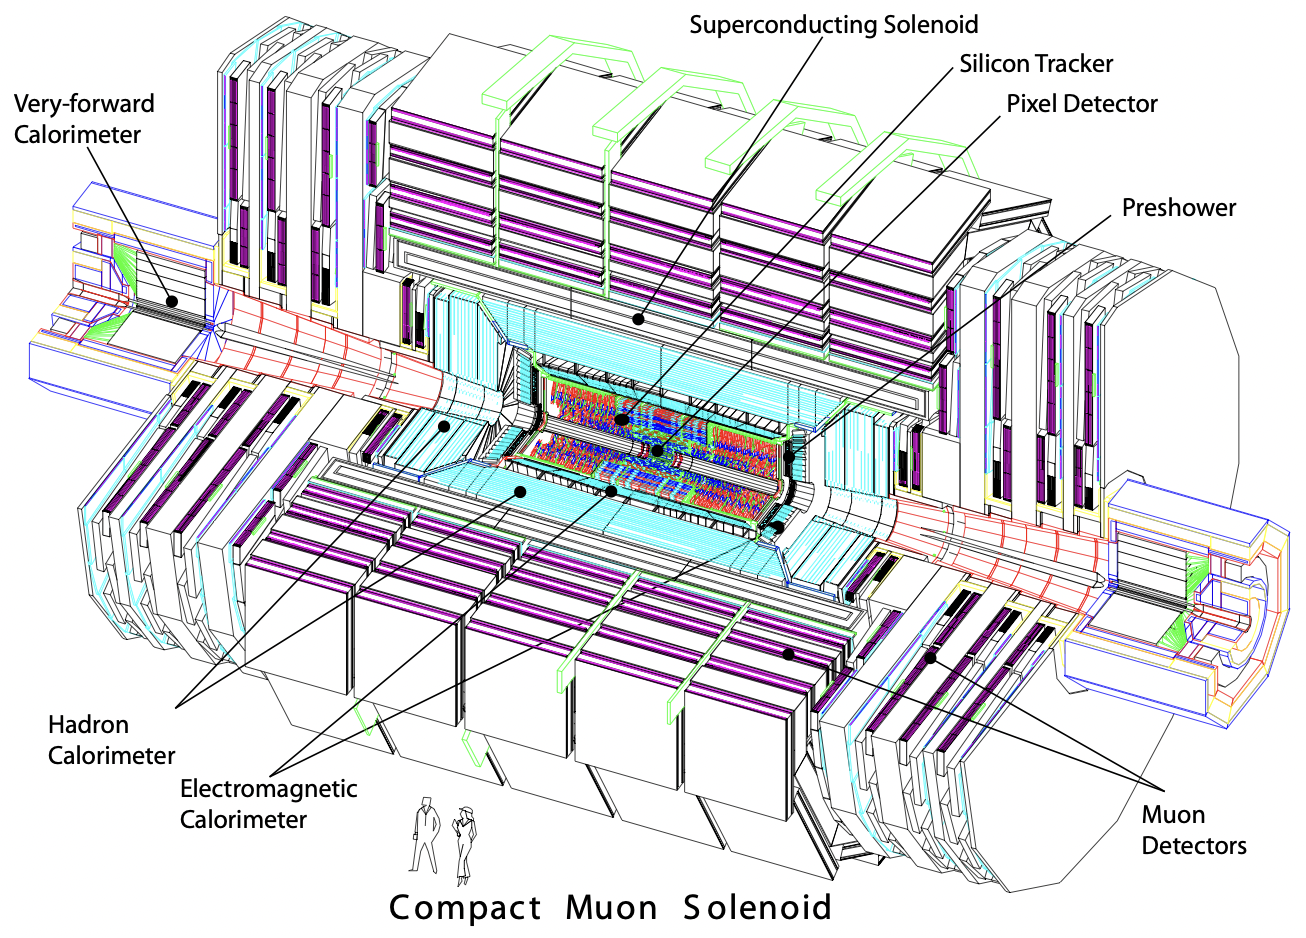
\includegraphics[width=0.6\textwidth]{figuras/CMS.png}
    \caption{A perspective view of the CMS detector \cite{CMS:2008}.}
    \label{fig:cms}
\end{figure}

\section{Data format and datasets}
\label{sec:dataset}

The CMS released reconstructed data in the CERN Open data format comes in a hierarchy of formats.
Each format sacrifices completeness for size making the choice of format the first decision required 
for an analysis using their datasets, since it fixes what information is available and what variables
are at hand. The three formats relevant here are summarised in
Table~\ref{tab:formats}.

\begin{table}[htbp]
    \centering
    \caption{The three CMS data-tier formats, in decreasing order of size and
    detail. Sizes are approximate and quoted relative to the baseline AOD.}
    \label{tab:formats}
    \begin{tabularx}{\textwidth}{@{}lXl@{}}
      \toprule
      Format & Content & Size \\
      \midrule
      AOD & High-level physics objects plus substantial lower-level
      reconstruction detail. & baseline \\[4pt]
      \midrule
      MiniAOD & Analysis-level physics objects similar to AOD but
      slimmed: many collections are reduced, extra information
      is packed into lighter objects, and less commonly used
      low-level detail is removed. &
            $\sim\!1/10$ of AOD \\[4pt]
        \midrule
      NanoAOD & Compact ntuple-style content: a limited set of per-object
      observables and precomputed IDs; little to no low-level
      detector detail (e.g., Particle Flow candidates dropped). &
            $\sim\!1/20$ of MiniAOD \\
      \bottomrule
    \end{tabularx}
\end{table}

For this work, the requirement is having access to the constituents of a jet. The substructure
observables of Chapter \ref{cap:estado-da-arte} are built by declustering a jet into its constituents,
so this analysis requires the individual particle-flow candidates that build the jet and not just 
a summary of the jet's kinematics. This immediality invalidates the NanoAOD data format since the particle-flow
candidates are not stored there. The AOD format stores the particle-flow candidates, however it also stores
other low-level reconstruction details which this analysis does not need making it occupy a large volume of
space. This leaves the MiniAOD data format, which occupies the middle ground of space and still
stores particle-flow candidates required for substructure while discarding the low-level information that is not
needed. Therefore, it is for this reason that the MiniAOD data format was the choice made for the format to be used
throughout this work.

Between all the MiniAOD datasets, this work analysed the JetHT primary dataset from the 2016 data-taking
period, in MiniAOD format~\cite{JetHT2016G}. Its characteristics are collected in
Table~\ref{tab:dataset}. The data are proton--proton collisions at a
centre-of-mass energy of $\sqrt{s} = 13$~TeV, recorded during run period G of 2016
and released as part of the Ultra-Legacy reprocessing, the final and most complete
calibration of the Run~2 data.

\begin{table}[htbp]
    \centering
    \caption{Characteristics of the JetHT primary dataset \cite{JetHT2016G}.}
    \label{tab:dataset}
    \begin{tabularx}{\textwidth}{@{}lX@{}}
      \toprule
      Property & Value \\
      \midrule
      Dataset & \texttt{/JetHT/Run2016G-UL2016\_MiniAODv2-v2/MINIAOD} \\
      Collision & proton--proton, $\sqrt{s} = 13$~TeV \\
      Run period & 2016G (runs 278820--280385) \\
      Events & $1.21 \times 10^{8}$ \\
      Size & 4.1~TiB (1236 files) \\
      \bottomrule
    \end{tabularx}
\end{table}
  
The JetHT dataset is well suited for this work analysis since it is enriched in jet events. CMS records
events online that pass a two-level trigger system, composed by a hardware Level-1 trigger followed by a software High Level Trigger
(HLT) \cite{CMS:2017trigger}. The events of this dataset are then those accepted by a set of HLT paths,
which require either a large scalar sum of jet transverse momenta
or the presence of one or two energetic jets. As a result the sample is dominated
by the high-transverse-momentum, high-multiplicity final states in which jet
substructure is most informative. Since the dataset is served by triggers based on large-radius jets, events are
required to pass one of the \texttt{HLT\_AK8PFJet} paths. The analysis is
restricted to jets with transverse momentum above $700$~GeV, where the
unprescaled paths of highest threshold, \texttt{HLT\_AK8PFJet450} and
\texttt{HLT\_AK8PFJet500}, are almost fully efficient. In this region any jet passing
the selection also satisfies these paths, so the trigger requirement introduces
no turn-on bias, and the sample sits in the hard, perturbative regime
motivated in Section~\ref{sec:qcd}.

Furthermore, as required for all analysis of this dataset, the data is restricted to a list of
runs certified as good physics, provided with the dataset release. So, events not in these
certified runs do not enter this analysis. In addition, jets in this released sample do not 
require any energy calibrations to be applied to them, since they already carry the standard jet energy corrections applied by CMS
in the Ultra-Legacy reprocessing.

Alongside the JetHT collision dataset, this analysis uses a simulated sample of QCD
multijet events. This is because the flavour of a splitting inside a jet cannot be accessed in data,
so it is not possible to determine the secondary splitting channel. What the simulation
provides is the set of generated partons, carrying flavour, which are clustered in the
same way as the reconstructed particles in data. First the partons are clustered into jets with the
anti-$\kt$ algorithm of section \ref{sec:antikt} and then, through the Cambridge/Aachen algorithm of Section
\ref{sec:ca} and the IFN algorithm of Section~\ref{sec:ifn}, into a branching
history in which each splitting acquires a flavour. It is from this process that 
the channel of each splitting, $g\to q\bar{q}$, $g\to gg$ or $q\to qg$, is labelled. 
This flavour labelling process and how it is further used in collision data is discussed in Section \ref{sec:flavour}. 
The sample used is a QCD multijet dataset generated with
\textsc{Pythia}~8~\cite{Sjostrand:2014zea} using the CP5
tune~\cite{CMS:2019csb}, passed through the full simulation of the CMS detector
and released in the same format as the collision data (MiniAODSIM)~\cite{QCDMC2016}.

\section{Analysis pipeline}
\label{sec:pipeline}

\section{Flavour selection}
\label{sec:flavour}

\section{Systematic uncertainties}
\label{sec:systematic}